\section{插图}
插图功能是利用 \TeX\ 的特定编译程序提供的机制实现的,不同的编译程序支持不同的图
形方式。有的同学可能听说“\LaTeX\ 只支持 EPS”,事实上这种说法是不准确的。\XeTeX\
可以很方便地插入 EPS、PDF、PNG、JPEG 格式的图片。

一般图形都是处在浮动环境中。之所以称为浮动是指最终排版效果图形的位置不一定与源文
件中的位置对应,这也是刚使用 \LaTeX\ 同学可能遇到的问题。如果要强制固定浮动图形
的位置,请使用 \pkg{float} 宏包,它提供了 \texttt{[H]} 参数。

\subsection{单个图形}
首先把你的图片放在本\LaTeX\ 项目的\texttt{figures}文件夹内,然后你可以通过指定图片的名称来这样插入,并且通过\texttt{ref}和\texttt{label}进行图片引用。如图~\ref{fig:cn100t} 所示。

\begin{figure}[h]
  	\centering
  	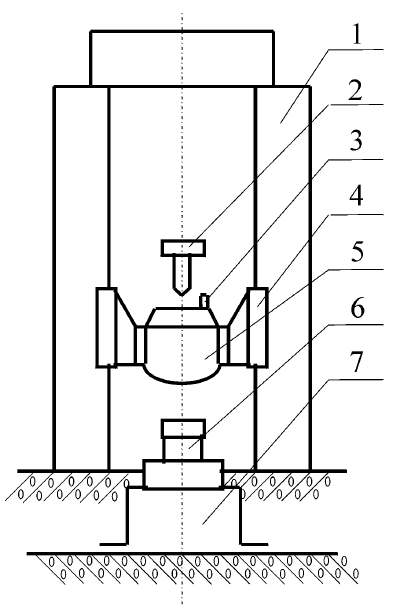
\includegraphics[width=4cm]{figures/cn100t.png}
	\caption{中文题图}
    \label{fig:cn100t}
\end{figure}

\subsection{多个图形}
简单插入多个图形的例子如图~\ref{fig:cn100t-2} 所示。这两个水平并列放置的子图共用一个
图形计数器,没有各自的子图题。

\begin{figure}[h]
  \centering
  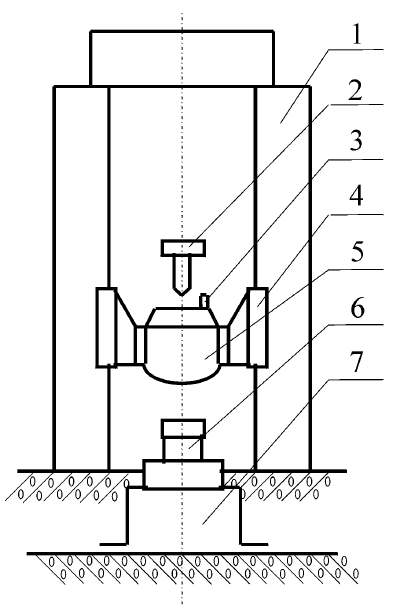
\includegraphics[height=4cm]{figures/cn100t.png}
  \hspace{1cm}
  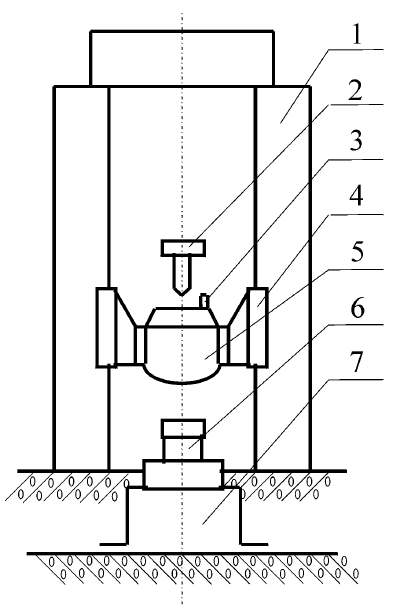
\includegraphics[height=4cm]{figures/cn100t.png}
  \caption{中文题图}
  \label{fig:cn100t-2}
\end{figure}


\section{表格}

\subsection{基本表格}
表格的编排建议采用国际通行的三线表\footnote{三线表,以其形式简洁、功能分明、阅读方便而在科技论文中被推荐使用。三线表通常只有 3 条线,即顶线、底线和栏目线,没有竖线。}。三线表可以使用 \pkg{booktabs} 提供的 \texttt{toprule}、\texttt{midrule} 和
\texttt{bottomrule}。它们与 \texttt{longtable} 能很好的配合使用。

\begin{table}[h]
  \caption{一个颇为标准的三线表}
  \label{tab:firstone}
  \centering
  \begin{tabular}{@{}llr@{}} \toprule
    \multicolumn{2}{c}{Item} \\ \cmidrule(r){1-2}
    Animal & Description & Price (\$)\\ \midrule
    Gnat  & per gram  & 13.65 \\
          & each      & 0.01 \\
    Gnu   & stuffed   & 92.50 \\
    Emu   & stuffed   & 33.33 \\
    Armadillo & frozen & 8.99 \\ \bottomrule
  \end{tabular}
\end{table}
\footnotetext{这个例子来自
  \href{https://mirrors.sjtug.sjtu.edu.cn/ctan/macros/latex/contrib/booktabs/booktabs.pdf}%
  {《Publication quality tables in LaTeX》}(\pkg{booktabs} 宏包的文档)。这也是
  一个在表格中使用脚注的例子,请留意与 \pkg{threeparttable} 实现的效果有何不
  同。}
